%%%%%%%%%%%%%%%%%%%%%%%%%%%%%%%%%%%%%%%%%%%%%%%%%%%%%%%%%%%
%\documentclass[xcolor=x11names,compress]{beamer}
\documentclass[xcolor=x11names, aspectratio=169, compress]{beamer}
%% General document
\usepackage{graphicx, subfig}
%% Beamer Layout
\useoutertheme[subsection=false,shadow]{miniframes}
\useinnertheme{default}
\usefonttheme{serif}
\usepackage{palatino}

%%%%%%% Mes Packages %%%%%%%%%%%%%%%%
%\usepackage[french]{babel}
\usepackage[T1]{fontenc}
\usepackage{color}
\usepackage{xcolor}
\usepackage{dsfont} % Pour indicatrice
\usepackage{url}
\usepackage{multirow}
\usepackage[normalem]{ulem}   % For strike out text

% Natbib for clean bibliography
\usepackage[comma,authoryear]{natbib}

%remove the icon
\setbeamertemplate{bibliography item}{}

%remove line breaks
\setbeamertemplate{bibliography entry title}{}
\setbeamertemplate{bibliography entry location}{}
\setbeamertemplate{bibliography entry note}{}

%% ------ MEs couleurs --------
\definecolor{vert}{rgb}{0.1,0.7,0.2}
\definecolor{brique}{rgb}{0.7,0.16,0.16}
\definecolor{gris}{rgb}{0.7, 0.75, 0.71}
\definecolor{twitterblue}{rgb}{0, 0.42, 0.58}
\definecolor{airforceblue}{rgb}{0.36, 0.54, 0.66}
\definecolor{siap}{RGB}{3,133, 200}


%%%%%%%%%%%%%%%%% BEAMER PACKAGE %%%%%%%

\setbeamercolor{itemize item}{fg=siap}
%\setbeamercolor{itemize subitem}{fg=blue}
%\setbeamercolor{itemize subsubitem}{fg=cyan}

\setbeamerfont{title like}{shape=\scshape}
\setbeamerfont{frametitle}{shape=\scshape}

\setbeamercolor*{lower separation line head}{bg=DeepSkyBlue4}
\setbeamercolor*{normal text}{fg=black,bg=white}
\setbeamercolor*{alerted text}{fg=siap}
\setbeamercolor*{example text}{fg=black}
\setbeamercolor*{structure}{fg=black}
\setbeamercolor*{palette tertiary}{fg=black,bg=black!10}
\setbeamercolor*{palette quaternary}{fg=black,bg=black!10}

% Set the header color to SIAP's color
\setbeamercolor*{frametitle}{fg=siap}

%remove navigation symbols
\setbeamertemplate{navigation symbols}{}

\renewcommand{\(}{\begin{columns}}
\renewcommand{\)}{\end{columns}}
\newcommand{\<}[1]{\begin{column}{#1}}
\renewcommand{\>}{\end{column}}

%% Add footer with logo
\setbeamertemplate{footline}{%
  \begin{beamercolorbox}[wd=\paperwidth,ht=2.5ex,dp=1.125ex,%
    leftskip=.3cm,rightskip=.3cm plus1fil]{author in head/foot}
    
\includegraphics[height=5ex]{SIAP_logo_Big.png}\hfill
    \insertshortauthor\hfill\insertshorttitle\hfill  \textcolor{siap}{\textit{\insertframenumber}}
  \end{beamercolorbox}%
}


% Path for the graphs
\graphicspath{
{Graphics/}
{../../../../Visualisation/Presentations/Graphics/Logos}
{../../Visualisation/Presentations/Graphics/}
{c:/Gitmain/MLCourse/UNML/Module0/M0_files/figure-html/}
{c:/Chris/UN-ESCAP/MyCourses2022/MLOS2022/Slides/Graphics/}
{c:/Chris/UN-ESCAP/MyCourses2023/BigDataKostat/Slides/Graphics/}
{../../../../Visualisation/Presentations/Graphics/SIAP/icons/}
{c:/Chris/UN-ESCAP/SIAP-E-learning/Resources/Pictos/}
{c:/Chris/UN-ESCAP/MyCourses2024/BigData/Slides/Graphics/}
 }

\title{\textcolor{siap}{Big Data and Data Science for Gender Statistics in Asia and the Pacific\\ \vspace{0.5cm} }}

\subtitle{\textcolor{brique}{\Large{Web Scraping With APIs}}}
\author{Christophe Bontemps}
\institute{ 
\includegraphics[height=10ex]{SIAP_logo_Big.png}}
\date{}

\begin{document}

% Slide 1: Title Slide
\begin{frame}
    \titlepage
\end{frame}

\section{What is an API?}

\begin{frame}{What is an API?}

\begin{columns}[T]
  \begin{column}{0.7\textwidth}
    \begin{itemize}[<+->]
        \item Sometimes data providers propose an efficient way to download data
        \item API: "\textbf{A}pplication \textbf{P}rogramming \textbf{I}nterface "
        \item An API is like a \textbf{robot waiter} in a restaurant
        \item[$\hookrightarrow$ ] He has a menu
        \item[$\hookrightarrow$ ] You can order anything but only on the Menu
        \item[$\hookrightarrow$ ] Data is then served as a structured "ready-to-use" file
     \end{itemize}
     \end{column}

    \begin{column}{0.3\textwidth}
    \begin{center}
      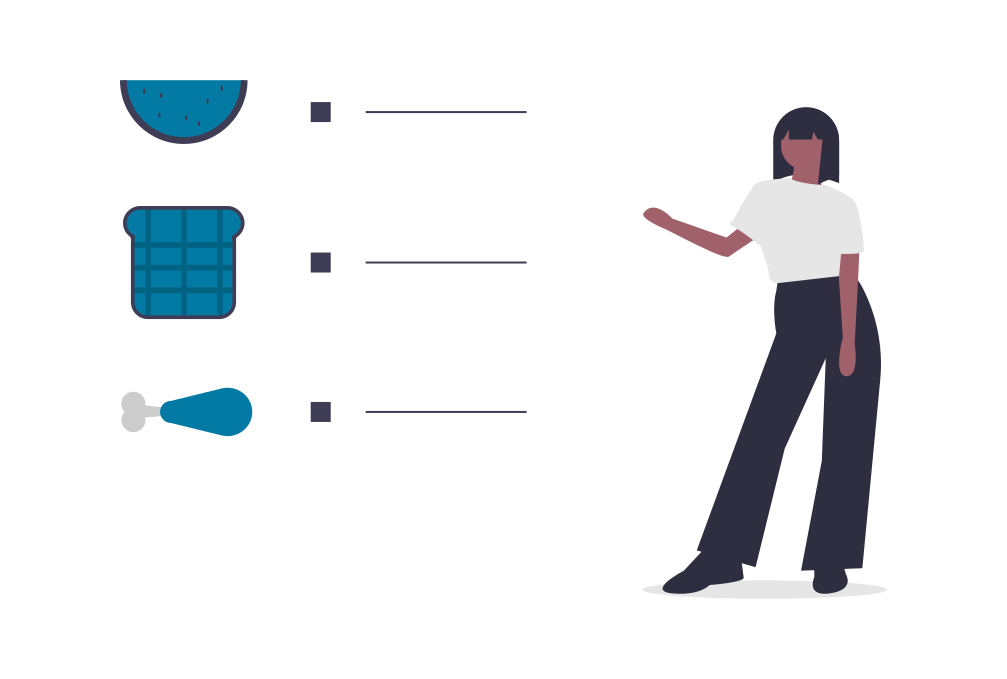
\includegraphics[width=0.9\textwidth]{undraw_diet_ghvw.png} \\
      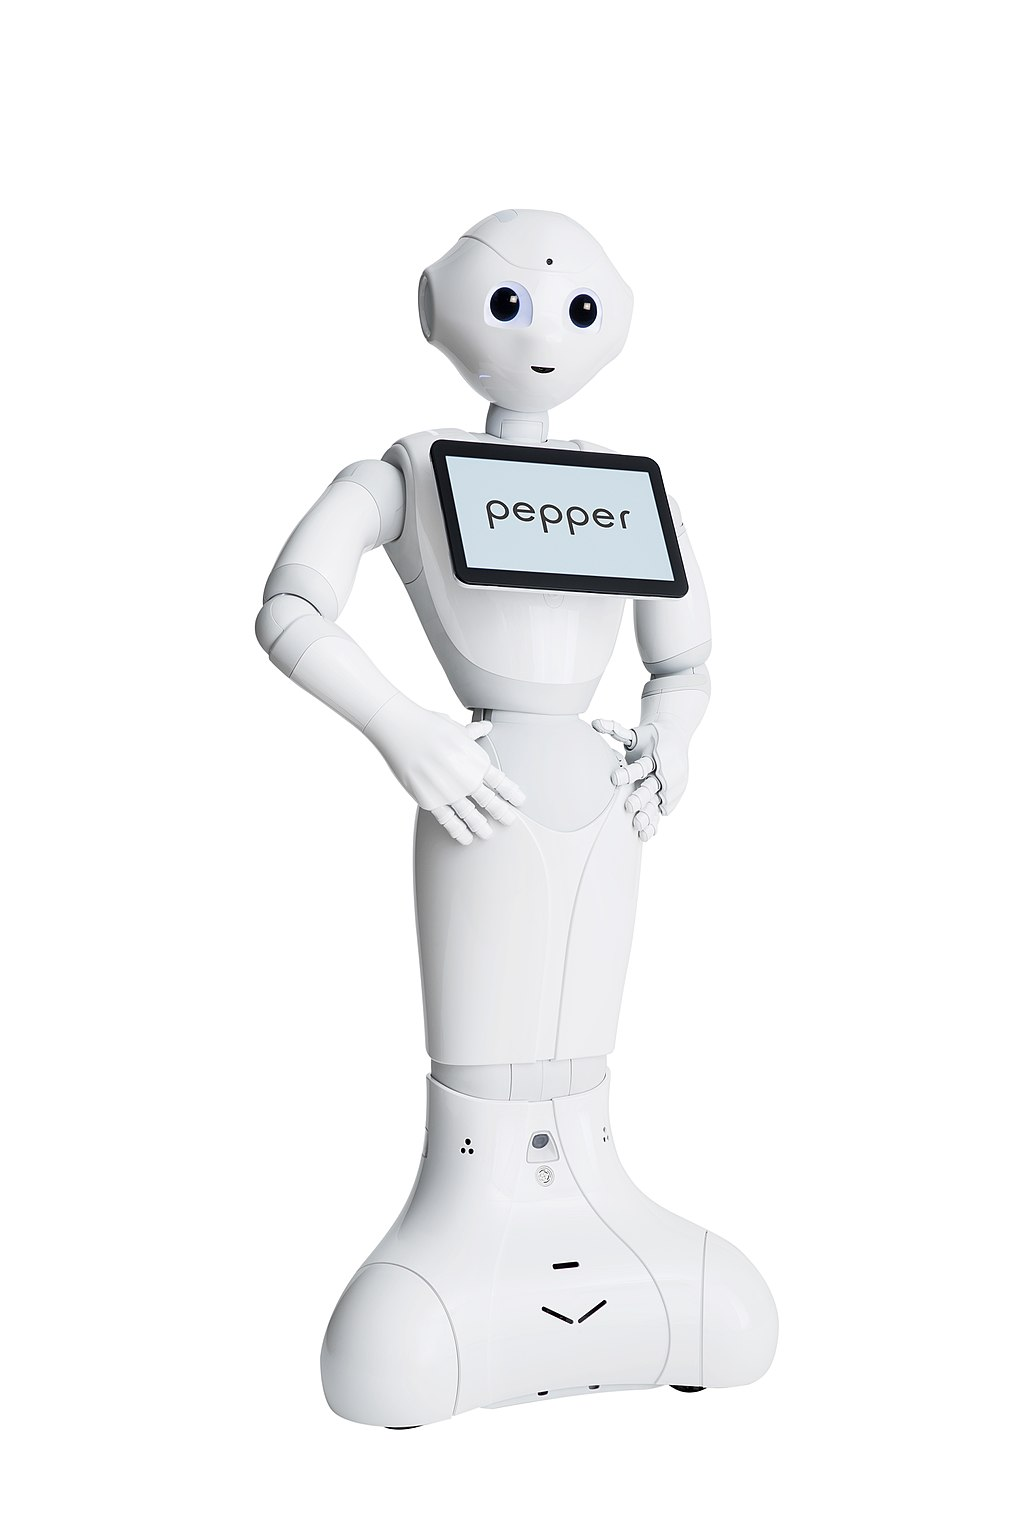
\includegraphics[width=0.9\textwidth]{Pepper_the_Robot.jpg} \\
      \textcolor{gris}{\tiny \href{https://commons.wikimedia.org/wiki/File:Pepper_the_Robot.jpg}{Source: Softbank Robotics Europe}}
    \end{center}
    \end{column}
\end{columns}
\end{frame}



\begin{frame}{Advantages of APIs}
\pause
\begin{enumerate}[<+->]
    \item Efficient
    \item Reliable
    \item Validated
    \item Legal
    \item Facilitated
\end{enumerate}
\end{frame}

\section{Case studies}

\subsection{WHO}

\begin{frame}{Collecting data from WHO}
\begin{columns}[T]
  \begin{column}{0.8\textwidth}
    \begin{itemize}[<+->]
        \item Use \href{https://www.who.int/data/gho/info/athena-api}{Athena API} web site
        \item Request follow a strict language:
        \item[] \small{\texttt{http://HOST[:PORT]/PATH/athena/INSTANCE/}}
        \item[] \small{\texttt{[DIMENSION[/CODE[,CODE2[,CODEn][.EXTENSION]]}}
        \item[] \small{\texttt{[?QUERY\_PARAMETERS]]]}}
        \item We have to read the instructions
        \item[ ] \small{\texttt{http://HOST[:PORT]/PATH/athena/}} $\hookrightarrow$ is the server
        \item[]\small{\texttt{[INSTANCE]}} $\hookrightarrow$ Is the \textbf{api} for us
        \item[]\small{\texttt{[DIMENSION[(..)]]}} $\hookrightarrow$ is list of available codes for a specific dimension
     \end{itemize}
     \end{column}

    \begin{column}{0.2\textwidth}
    \begin{center}
      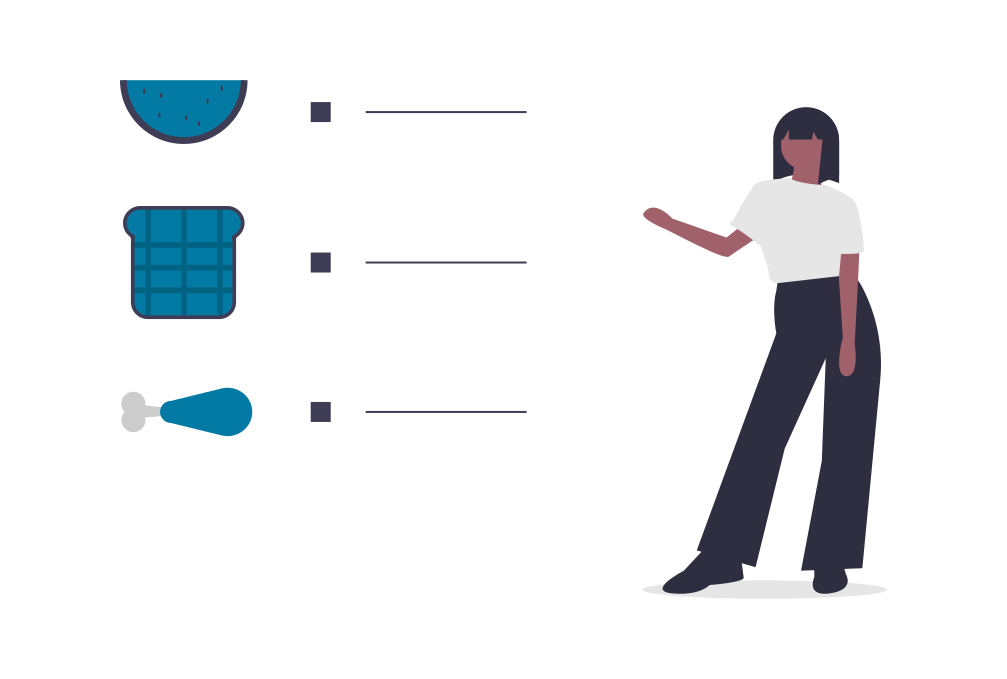
\includegraphics[width=0.9\textwidth]{undraw_diet_ghvw.png}
    \end{center}
    \end{column}
\end{columns}
\end{frame}


\begin{frame}{Example 1: Collecting data from WHO}
\begin{columns}[T]
  \begin{column}{0.8\textwidth}
    \begin{itemize}[<+->]
       \item Finally
       \item[]\small{\texttt{[?QUERY\_PARAMETERS]}} $\hookrightarrow$ Is where we select things!
       \item Example:
       %\item[]\small{\texttt{WHOSIS\_000001??filter=COUNTRY:BWA;YEAR:2011;SEX:BTSX}}
       \item[]\small{\texttt{\textcolor{brique}{WHOSIS\_000001}??filter=\textcolor{siap}{COUNTRY:BWA};\textbf{YEAR:2011};\textcolor{vert}{SEX:BTSX}}}
       \item[$\hookrightarrow$ ] Means
        \item[]\texttt{\textcolor{brique}{WHOSIS\_000001}} is the target we use to request the data regarding Life expectancy at birth.
        \item[]\texttt{\textcolor{siap}{COUNTRY:BWA}} Filter by country  code for Botswana,
        \item[]\texttt{\textbf{YEAR:2011}} Filter on the year 2011.
         \item[]\texttt{\textcolor{vert}{SEX:BTSX}} Both Sex
     \end{itemize}
     \end{column}

    \begin{column}{0.2\textwidth}
    \begin{center}
      \href{https://www.who.int/data/gho/info/athena-api}{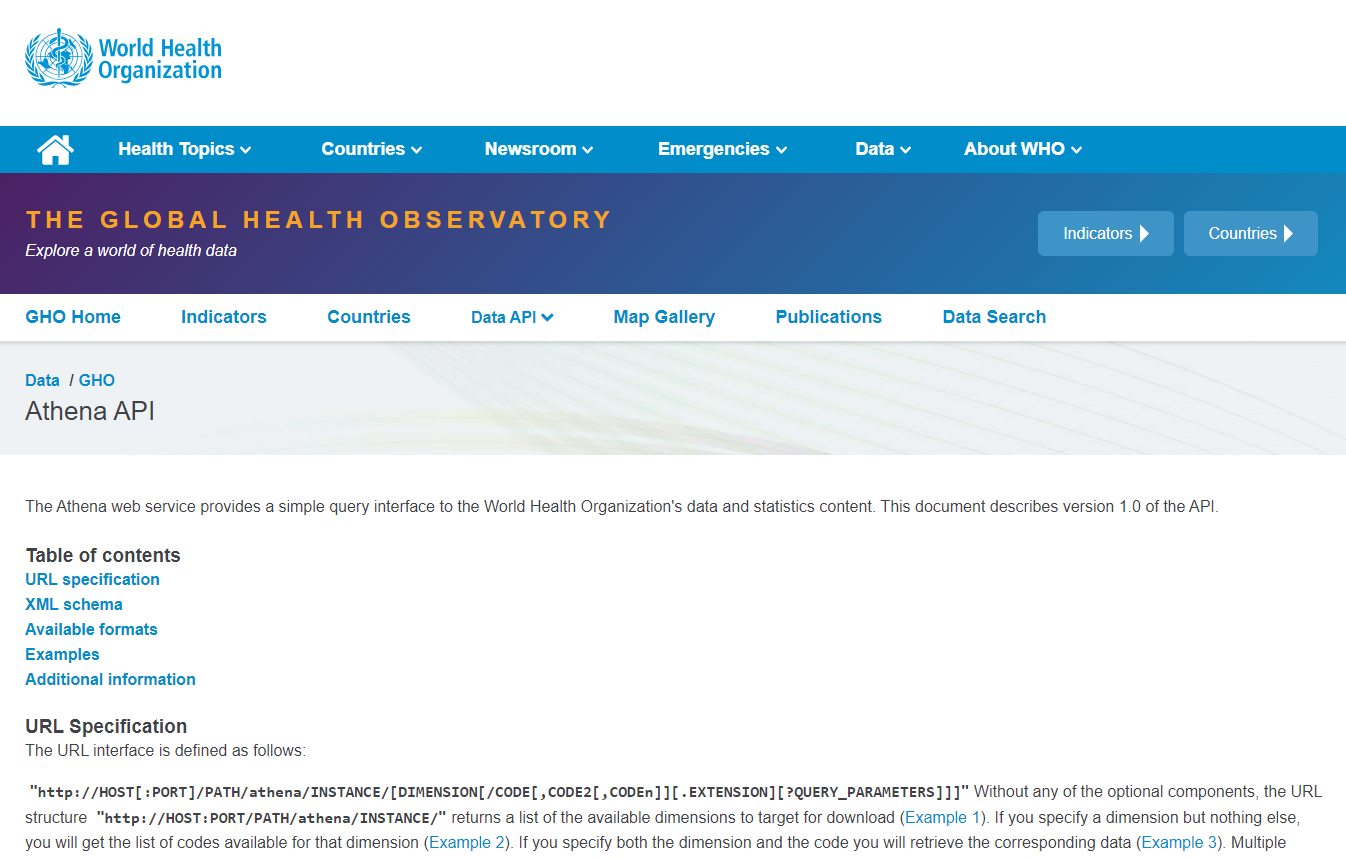
\includegraphics[width=0.9\textwidth]{WHO_API.PNG}}
    \end{center}
    \end{column}
\end{columns}
\end{frame}

\begin{frame}{Collecting data from WHO}
\begin{columns}[T]
  \begin{column}{0.2\textwidth}
    \begin{itemize}[<+->]
       \item[] Details

     \end{itemize}
     \end{column}

    \begin{column}{0.8\textwidth}
    \begin{center}
      \begin{itemize}
    \only<1>{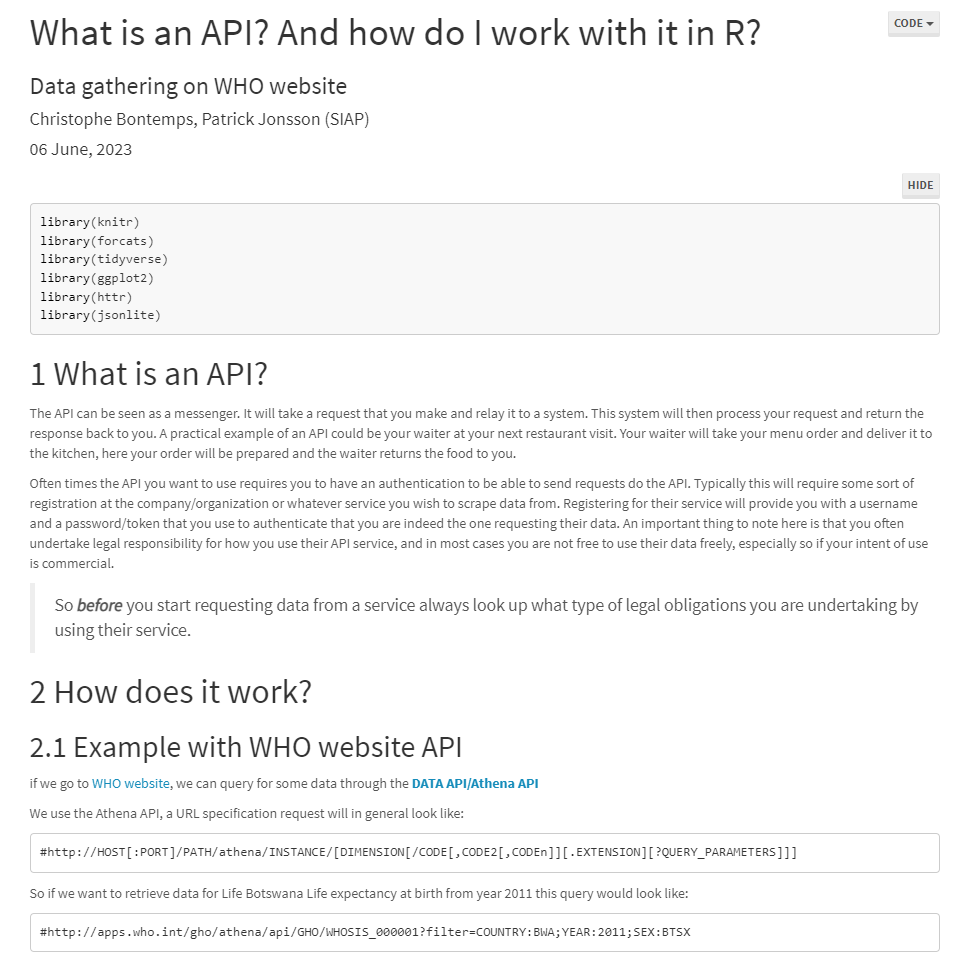
\includegraphics[width=0.9\textwidth]{ApiSlides1.png}  \\ }
    \only<2>{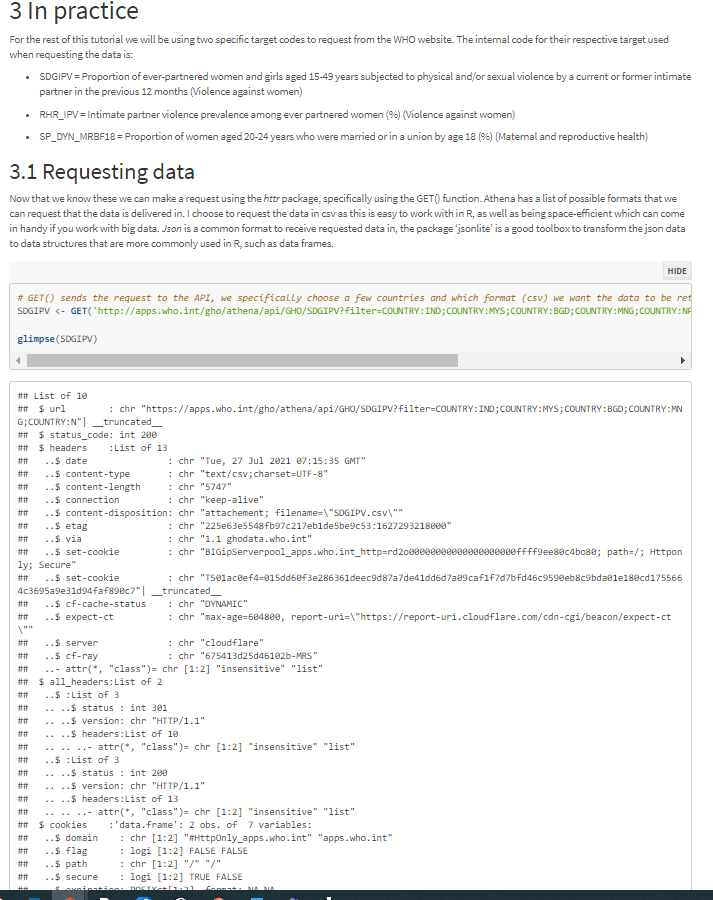
\includegraphics[width=0.9\textwidth]{ApiSlides2.png}  \\ }
    \only<3>{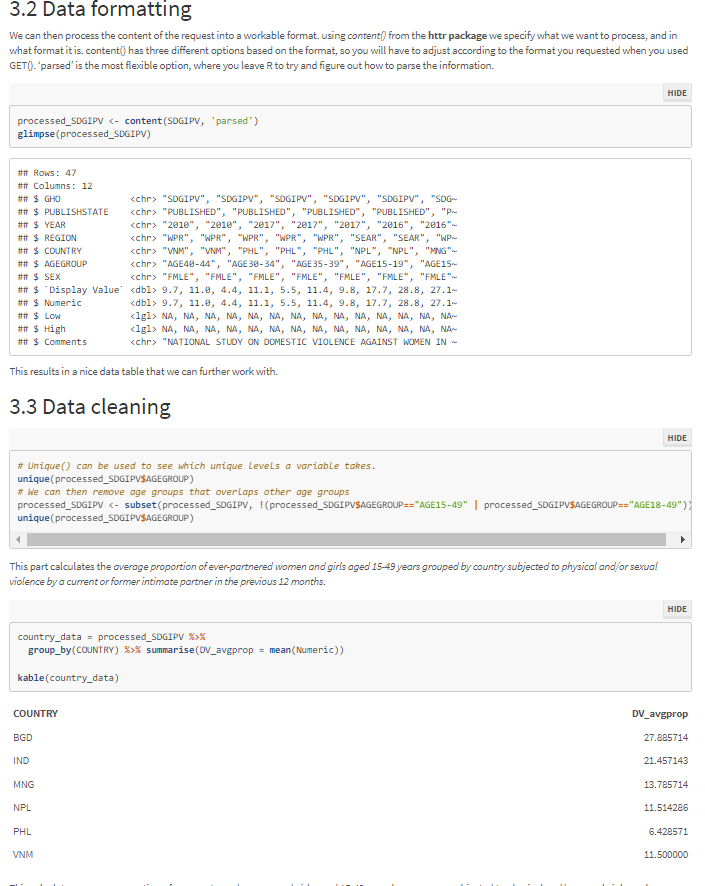
\includegraphics[width=0.9\textwidth]{ApiSlides3.png}  \\ }
    \only<4>{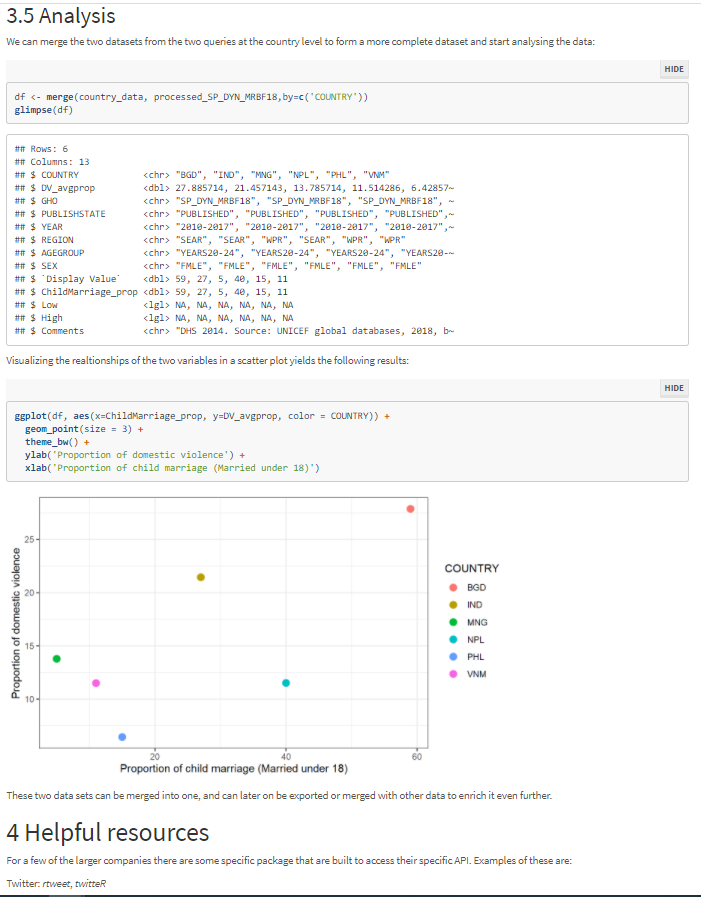
\includegraphics[width=0.9\textwidth]{ApiSlides4.png}  \\ }

   \end{itemize}
    \end{center}
    \end{column}
\end{columns}
\end{frame}

\subsection{GFW}

\begin{frame}{Example 2: Global Fishing Watch }
\begin{columns}[T]
  \begin{column}{0.6\textwidth}
Sequence
\begin{itemize}[<+->]
    \item Read the instruction for \href{https://globalfishingwatch.org/our-apis/documentation}{GFW API}
    \begin{enumerate}[<+->]
    \item Register for a Global Fishing Watch account.
    \item Request an API Access Token
    \item Agree to the terms of use (cite Global Fish Watch as source)
\end{enumerate}
    \item Construct a request
    \item[$\hookrightarrow$ ] Search a fishing vessel and get the fishing events / port returns
     \item Analyze and visualize
\end{itemize}
     \end{column}
    \begin{column}{0.4\textwidth}
    \begin{center}
      \begin{itemize}
    \only<1-4>{\href{https://globalfishingwatch.org/our-apis/documentation}{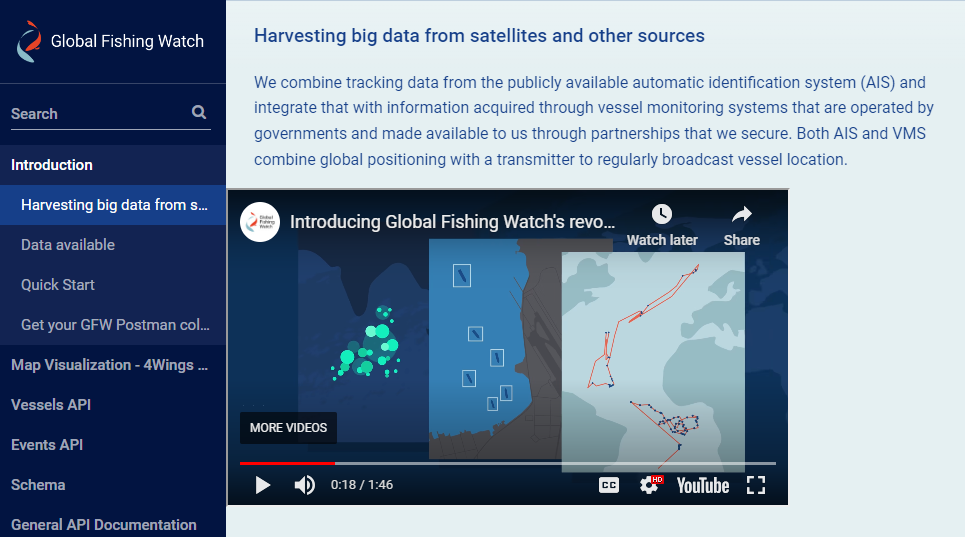
\includegraphics[width=0.9\textwidth]{GFWPage.PNG}}  \\ }
    \only<3-4>{ \vspace{0.5cm} 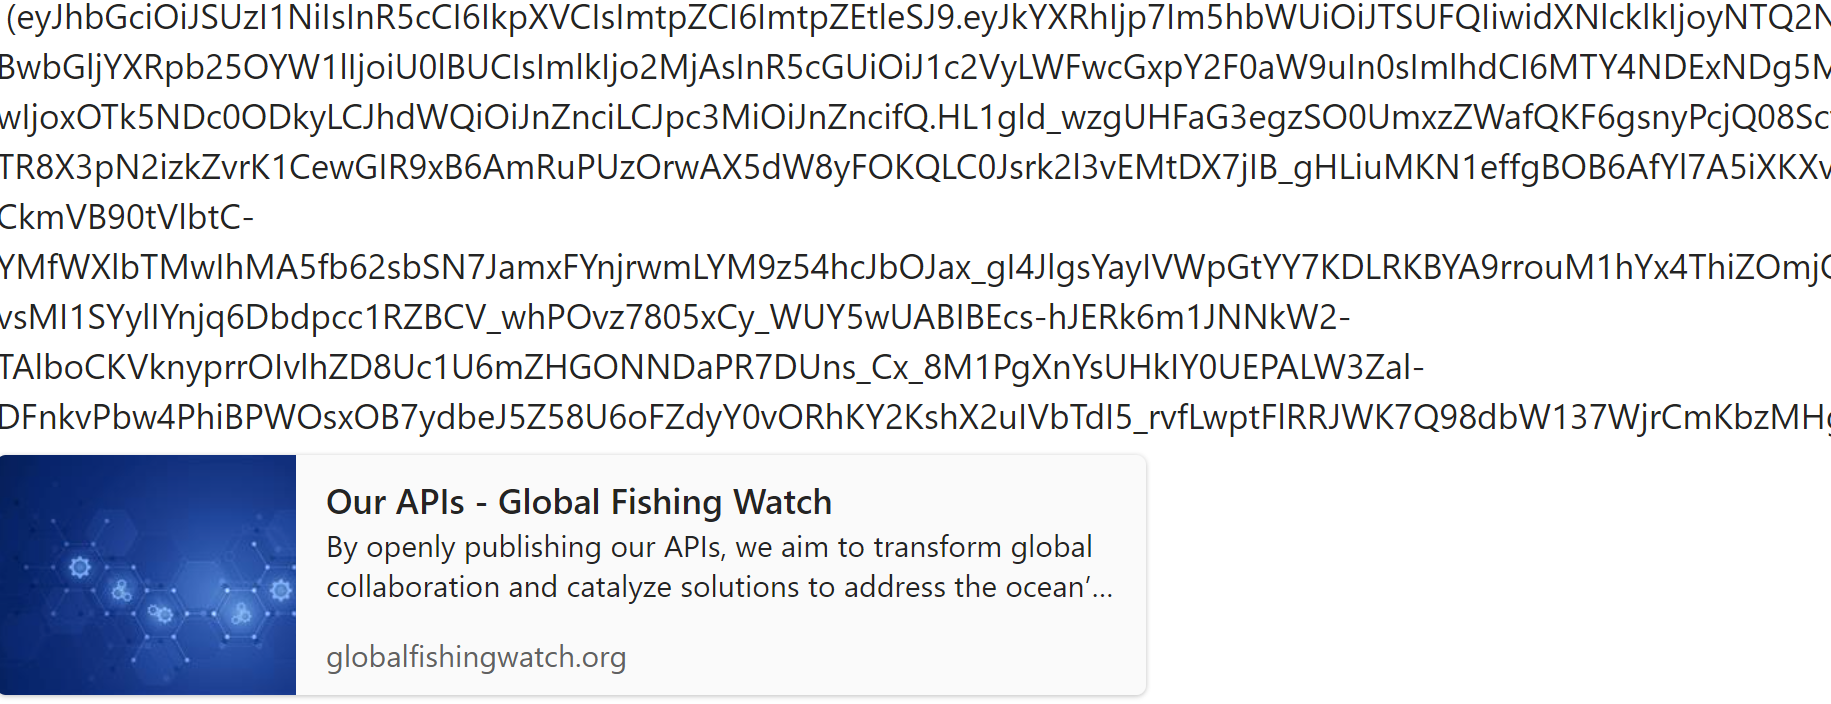
\includegraphics[width=0.8\textwidth]{GFWToken.PNG}  \\ }
    \only<5-6>{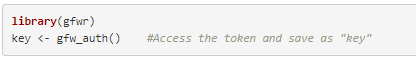
\includegraphics[width=\textwidth]{GFWStep1.PNG}  \\ }
    \only<5-6>{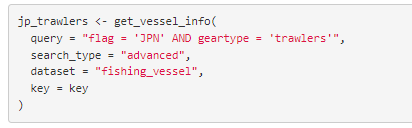
\includegraphics[width=\textwidth]{GFWStep2.PNG}  \\ }
    \only<6>{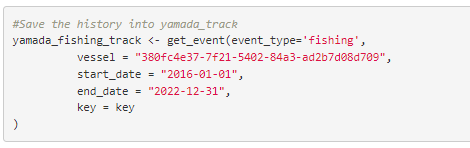
\includegraphics[width=\textwidth]{GFWStep3.PNG}  \\ }
    \only<7>{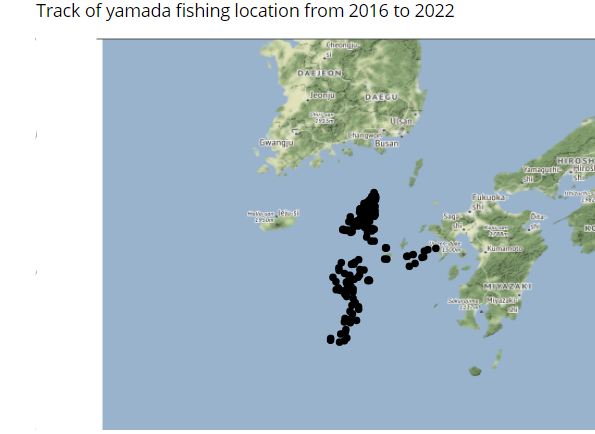
\includegraphics[width=\textwidth]{GFWStep4.PNG}  \\ }
    \only<8>{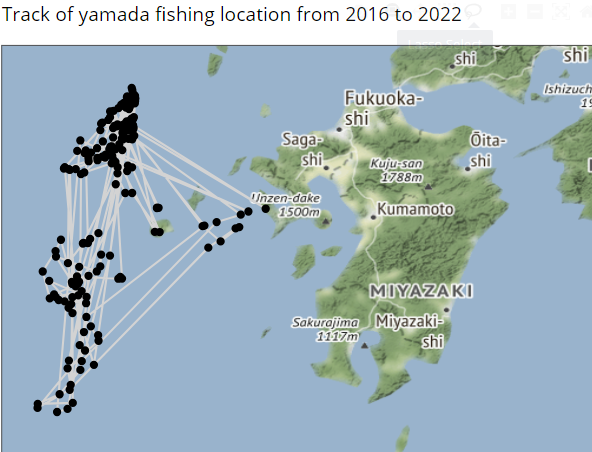
\includegraphics[width=\textwidth]{GFWStep5.PNG}  \\ }
    \only<9>{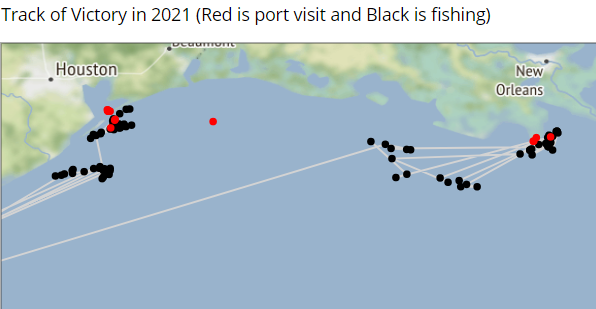
\includegraphics[width=\textwidth]{GFWStep6.PNG}  \\ }

   \end{itemize}
    \end{center}
    \end{column}
\end{columns}
\end{frame}



\begin{frame} % Cover slide
\frametitle{\textcolor{brique}{[Q\&A]}}
\begin{center}
\Large \textcolor{siap}{ Questions}
\end{center}
\end{frame}


\end{document}


\begin{frame} % Cover slide
\frametitle{ }
\pause
 \begin{itemize}[<+->]
  \item[]
  \item
\end{itemize}
\end{frame}

%%%%%%%%%%%%%%% Last Slide %%%%%%%%%%%%%%%%

\begin{frame}[allowframebreaks]%in case more than 1 slide needed
\frametitle{References}
    {\footnotesize
    %\bibliographystyle{authordate1}
    \bibliographystyle{apalike}
    \bibliography{../../../Visualisation/Visu}
    }
\end{frame}
\end{document}

%\bibliographystyle{authordate1}
%\bibliography{c:/Chris/Visualisation/Visu}
%\end{frame}

\begin{frame}{Title}
\begin{columns}[T]
  \begin{column}{0.7\textwidth}
    \begin{itemize}[<+->]
        \item Sometimes data providers propose a more efficient way to download data
        \item API: "\textbf{A}pplication \textbf{P}rogramming \textbf{I}nterface "
        \item An API is like a waiter in a restaurant
        \item[$\hookrightarrow$ ] He has a menu
        \item[$\hookrightarrow$ ] You can order anything but only on the Menu
        \item[$\hookrightarrow$ ] Data is then served as a structured "ready-to-use" file
     \end{itemize}
     \end{column}

    \begin{column}{0.3\textwidth}
    \begin{center}
      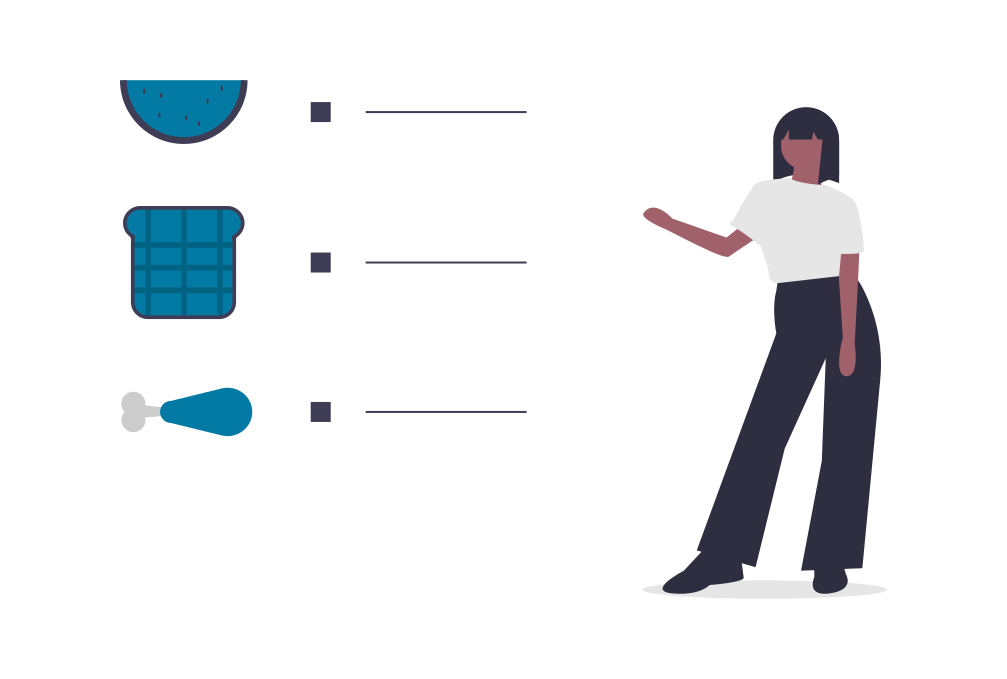
\includegraphics[width=0.9\textwidth]{undraw_diet_ghvw.png}
    \end{center}
    \end{column}
\end{columns}
\end{frame}

